% sample: clutter rate=50, sample no. 097

Finally, we evaluate tracking results for the similar case as (C3) but with external information fusion. The tracking scenario with estimates generated by the GM-PHD filter is illustrated in Figure \ref{fig:c4-results-overview}. We can see that the filter now detects new targets and the estimates are precise even though the initial mean vectors and covariance matrices are not precise. 

\begin{figure*}
    \centering
    \begin{subfigure}[]{0.48\linewidth}
        \centering
        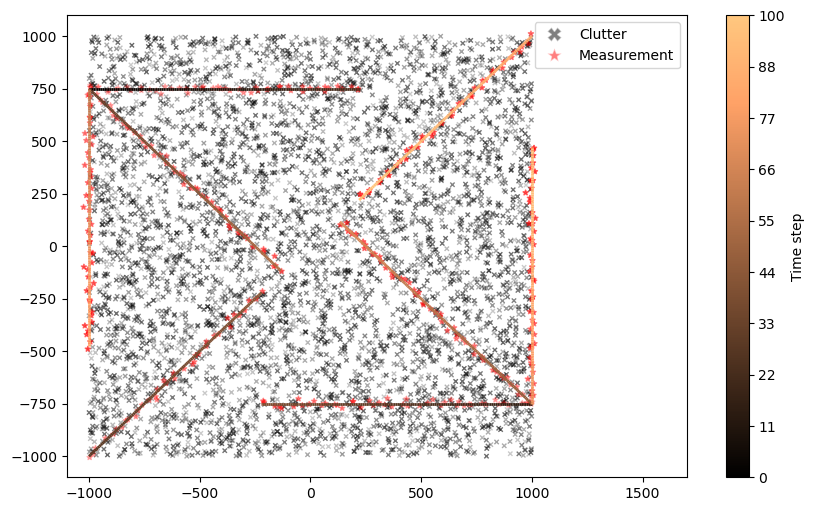
\includegraphics[width=\linewidth]{figures/c4-tracks-measurements.png}
    \end{subfigure}
    \hfill
    \begin{subfigure}[]{0.48\linewidth}
        \centering
        \begin{subfigure}[t]{\linewidth}
            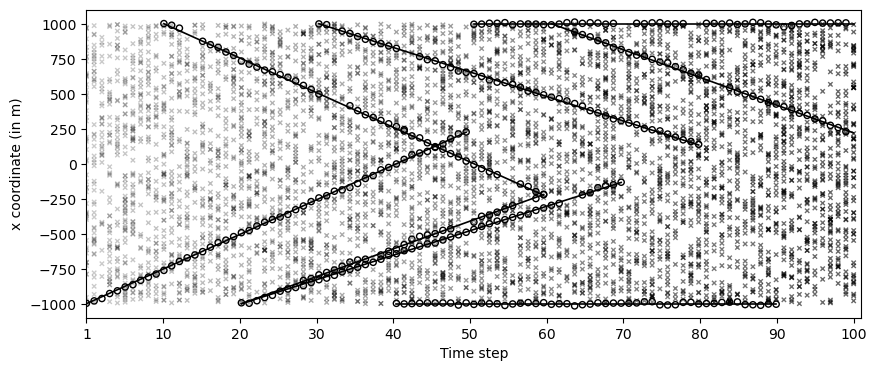
\includegraphics[width=\linewidth]{figures/c4-x-estimates.png}
        \end{subfigure}
        \vfill\par
        \begin{subfigure}[b]{\linewidth}
            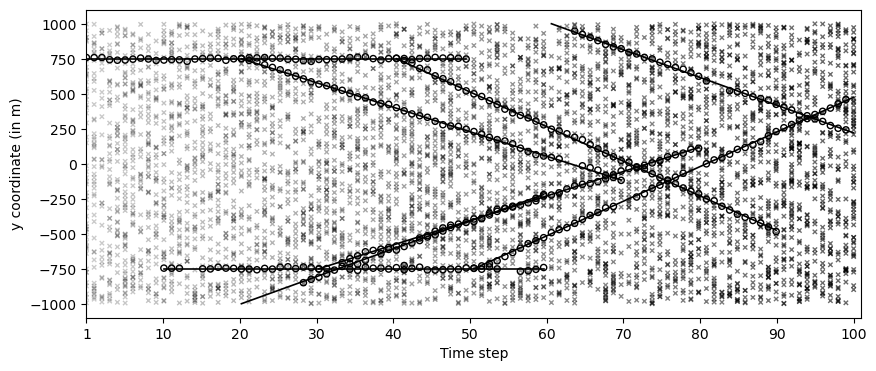
\includegraphics[width=\linewidth]{figures/c4-y-estimates.png}
        \end{subfigure}
    \end{subfigure}
  \caption[One sample of data and estimates for the (C4) scenario.]{One sample of data and estimates for the (C4) scenario. Left: True tracks of two objects (black to yellow) with clutter measurements (gray crosses) and received measurements (red stars) for a single Monte Carlo sample. Right: Change of both coordinates in time with noise measurements (red circles) and filter estimates (black circles) for the same Monte Carlo sample. Two targets were not detected by the filter, and no estimates were generated for them.}
  \label{fig:c4-results-overview}
\end{figure*}

In Figure \ref{fig:c4-traj-post}, we see the same track continuity problem, where the filter created nine trajectories, while there are only eight targets. However, in comparison to the (C3) scenario, the objects are now detected, and their tracks are estimated correctly. Despite trajectory estimates being present, note that the filter required some time to start detecting the the bottom-left target. It is due to its large uncertainty and the small weight, their exact values are given in Section \ref{sec:c4-scenario}. Thus, the GM-PHD algorithm required several additional measurements to confirm the track.

\begin{figure}
    \centering
    \begin{subfigure}[]{0.48\linewidth}
        \centering
        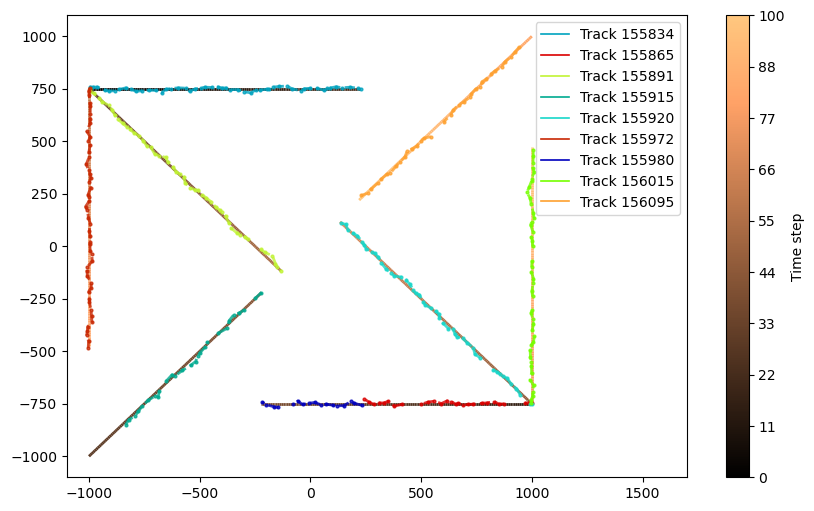
\includegraphics[width=\linewidth]{figures/c4-traj.png}
    \end{subfigure}
    \hfill
    \begin{subfigure}[]{0.48\linewidth}
        \centering
        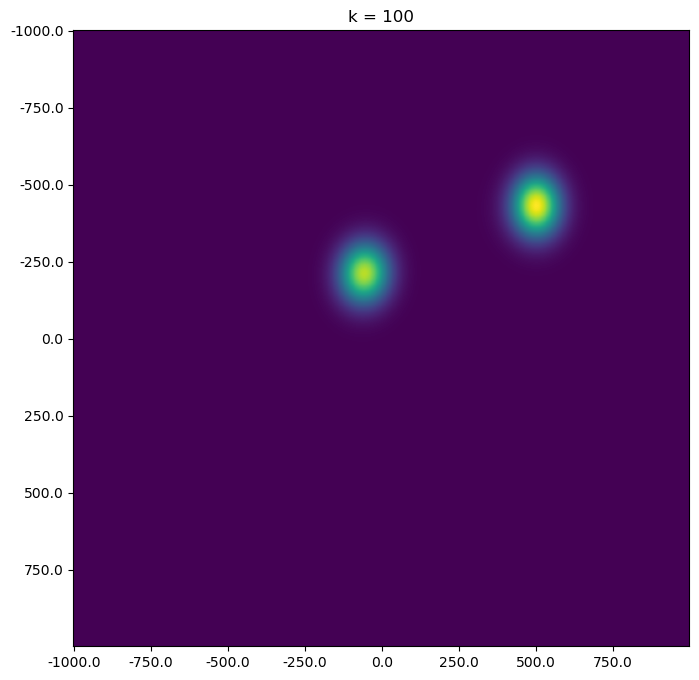
\includegraphics[width=\linewidth]{figures/c4-post.png}
    \end{subfigure}
  \caption[(C4). Trajectories estimations and the posterior intensity.]{Left: The visualization of trajectories estimates and the posterior distribution at time $k=100$. In comparison to the (C3) scenario, two targets are now detected correctly. Right: The posterior distribution at time step $k=100$. We see two Gaussian components that refer to two existing objects. For visualization purposes, the covariance matrices of all Gaussian components were multiplied by the factor of $81$. The filter was run with default settings, i.e. $\lambda_{c} = 12.5 \times 10^{-6}$, $P_{D,k} = 0.98$, $P_{S,k} = 0.99$, $\tau = 10^{-5}$, and $U=4$.}
  \label{fig:c4-traj-post}
\end{figure}

The visualization of all metrics for different filter settings is included in Appendix \ref{appendix:results-figures}. Here, we compare the evaluation of these metrics for default parameters in scenarios (C3) and (C4), as shown in Table \ref{table:c3-c4-metrics}.

\begin{table}
\begin{center}
\begin{tabular}{ | c || c | c | }
    \hline
            & CPEP              & EAE               \\ [0.5ex]
    \hline\hline
    (C3)    & 0.87876           & 0.85900           \\ 
    (C4)    & \textbf{0.85900}  & \textbf{0.35380}  \\ [1ex]
    \hline
\end{tabular}
\end{center}
\caption[Comparison of simulation results for the (C3) and (C4) scenarios.]{The comparison of CPEP and the expected absolute error on the number of targets (EAE) for the scenarios (C3) and (C4). The numbers represent the averaged values of metrics over $100$ Monte Carlo samples. The filter was run with default settings, i.e. $\lambda_{c} = 12.5 \times 10^{-6}$, $P_{D,k} = 0.98$, $P_{S,k} = 0.99$, $\tau = 10^{-5}$, and $U=4$.}\label{table:c3-c4-metrics}
\end{table}
